\chapter{METODOLOGI}
\label{chap:metodologi}

% Ubah bagian-bagian berikut dengan isi dari desain dan implementasi

Penelitian ini dilaksanakan sesuai dengan desain sistem berikut dengan implementasinya.
Desain sistem merupakan konsep dari pembuatan dan perancangan keseluruhan sistem yang diwujudkan dalam blok-blok alur yang harus dikerjakan. 
Implementasi merupakan pelaksanaan teknis dari setiap blok yang ada pada desain sistem.

\section{Desain Sistem}
\label{sec:Desain Sistem}
Sistem yang dibuat pada tugas akhir ini merupakan implementasi dari konsep Algoritma Genetika yang merupakan teknik pencarian dengan memanfaatkan proses seleksi alamiah yang dikenal dengan proses evolusi.
Desain sistem secara keseluruhan dapat dilihat pada Gambar \ref{fig:metodologi}
\begin{figure} [ht] \centering
  % Nama dari file gambar yang diinputkan
  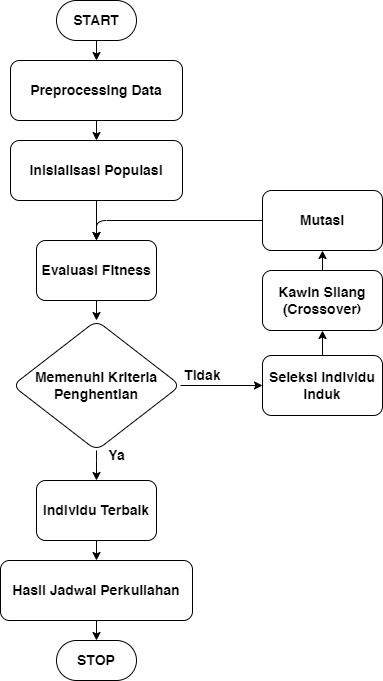
\includegraphics[scale=0.55]{gambar/desain.png}
  % Keterangan gambar yang diinputkan
  \caption{Desain Keseluruhan Sistem}
  % Label referensi dari gambar yang diinputkan
  \label{fig:metodologi}
\end{figure}

Agar sistem yang dibuat dapat mencapai tujuan yang telah ditentukan, maka sistem harus mengikuti rancangan yang tela ditentukan.
Pada Gambar \ref{fig:metodologi} dapat dilihat bahwa terdapat 2 proses penting yaitu preprocessing data dan proses algoritma genetika itu sendiri.
Pada proses preprocessing data dilakukan pengumpulan data-data yang diperlukan berupa data mata kuliah, dosen, ruangan dan waktu perkulihaan, desain kromosom yang digunakan, dan proses pengkodean gen.
Setelah kromosom dan data siap, proses selanjutnya adalah proses algoritma genetika yang terdiri atas inisialisasi populasi, evaluasi fitness, seleksi, crossover, dan mutasi.
Pada proses algoritma genetika, terdapat kondisi yang menghentikan seluruh proses algoritma genetika yang disebut dengan kriteria penghentian.
Jika terdapat individu yang memenuhi kriteria penghentian, individu tersebut dijadikan individu terbaik yang kemudian dapat diterjemahkan dalam bentuk tabel jadwal perkuliahan untuk satu pekan.

\subsection{Preprocessing Data}
  
  Preprocessing data pada penelitian ini meliputi proses pengumpulan data, desain kromosom, dan pengkodean kromosom. Pada penelitian ini, penulis akan menggunakan data dari Departemen Teknik Komputer ITS yang meliputi data mata kuliah, 
  jumlah ruangan, kapasitas masing-masing ruangan, jumlah dosen, dan jumlah mahasiswa pada tiap mata kuliah. Data-data tersebut antara lain:
  \begin{longtable}{|c|l|}
    \caption{Dosen Departemen Teknik Komputer ITS}
    \label{tb:DosenTekkom} \\
    \hline
    \rowcolor[HTML]{C0C0C0} 
    No. & Dosen                                         \\ \hline
    1   & Dr. Eko Mulyanto Yuniarno, S.T.,M.T.          \\ 
    2   & Dr. Diah Puspito Wulandari, S.T.,M.Sc.        \\ 
    3   & Dr. I Ketut Eddy Purnama, S.T.,M.T.           \\ 
    4   & Ir. Hany Boedinugroho, M.T.                   \\ 
    5   & Prof. Dr. Ir. Yoyon Kusnendar Suprapto, M.Sc. \\ 
    6   & Prof. Dr. Ir. Mauridhi Hery Purnomo, M.Eng.   \\ 
    7   & Dr. Surya Sumpeno, S.T.,M.Sc.                 \\ 
    8   & Eko Pramunanto, S.T., M.T.                    \\ 
    9   & Arief Kurniawan, S.T., M.T.                   \\ 
    10  & Muhtadin, S.T., M.T.                          \\ 
    11  & Atar Fuady Babgei, S.T., M.Sc.                \\ 
    12  & Mochamad Hariadi, S.T.,M.Sc.,Ph.D             \\ 
    13  & Dr. Supeno Mardi Susiki Nugroho, S.T., M.T.   \\ 
    14  & Susi Juniastuti, S.T.,M.Eng.                  \\ 
    15  & Ahmad Zaini, S.T., M.Sc.                      \\ 
    16  & Reza Fuad Rachmadi, S.T.,M.T.,Ph.D            \\ 
    17  & Dion Hayu Fandiantoro, S.T., M.Eng.           \\ 
    \hline
  \end{longtable}

\begin{longtable}{|c|l|r|}
  \caption{Mata Kuliah Semester Genap 2022-2023 \linebreak Departemen Teknik Komputer ITS}
  \label{tb:matkul}\\
  \hline
  \rowcolor[HTML]{D0CECE} 
  No. & Mata Kuliah & Peserta \\ \hline
  1  & Aljabar Linear - A                            & 5  \\
  2  & Arsitektur dan Organisasi Sistem Komputer - A & 30 \\
  3  & Arsitektur dan Organisasi Sistem Komputer - B & 27 \\
  4  & Dasar Pemrograman - P                         & 14 \\
  5  & Deep Learning untuk Multimedia - A            & 19 \\
  6  & Desain dan Pemrograman Game - A               & 9  \\
  7  & Desain dan Pemrograman Game - P               & 8  \\
  8  & Desain Dan Rekayasa Sistem - A                & 49 \\
  9  & Desain Dan Rekayasa Sistem - B                & 40 \\
  10 & Jaringan Komputer - A                         & 41 \\
  11 & Jaringan Komputer - B                         & 40 \\
  12 & Matematika Diskrit - A                        & 32 \\
  13 & Matematika Diskrit - B                        & 59 \\
  14 & Metode Numerik - A                            & 40 \\
  15 & Metode Numerik - B                            & 40 \\
  16 & Metode Numerik - C                            & 59 \\
  17 & Pemrograman Lanjut - A                        & 39 \\
  18 & Pemrograman Lanjut - B                        & 39 \\
  19 & Pemrograman Sistem dan Jaringan - A           & 11 \\
  20 & Pengantar Robotika - A                        & 33 \\
  21 & Pengolahan Sinyal Digital - A                 & 26 \\
  22 & Pengolahan Sinyal Digital - B                 & 26 \\
  23 & Persamaan Differensial dan Deret - A          & 35 \\
  24 & Persepsi Robot - A                            & 13 \\
  25 & Probabilitas dan Statistik - A                & 28 \\
  26 & Rangkaian Digital - A                         & 24 \\
  27 & Rangkaian Listrik - A                         & 40 \\
  28 & Rangkaian Listrik - B                         & 35 \\
  29 & Sekuriti Sistem Komputer - A                  & 33 \\
  30 & Sistem Manajemen Basis Data - A               & 25 \\
  31 & Sistem Manajemen Basis Data - B               & 25 \\
  32 & Sistem Mikroprosesor dan Mikrokontroller - A  & 26 \\
  33 & Sistem Mikroprosesor dan Mikrokontroller - B  & 20 \\
  34 & Sistem Operasi - A                            & 25 \\
  35 & Sistem Operasi - B                            & 26 \\
  36 & Sistem Tertanam - A                           & 27 \\
  37 & Sistem Tertanam - B                           & 24 \\
  38 & Visi Komputer - A                             & 16 \\    
  \hline
\end{longtable}

\begin{longtable}{|c|l|r|}
  \caption{Ruang Kelas Departemen Teknik Komputer ITS}
  \label{tb:ruang}\\
  \hline
  \rowcolor[HTML]{D0CECE} 
  No. & Ruangan & Kapasitas \\ \hline
  1   & A108                                                 & 80                                                     \\ 
  2   & A234                                                 & 36                                                     \\ 
  3   & A235                                                 & 40                                                     \\ 
  4   & AJ401                                                & 25                                                     \\ 
  5   & AJ402                                                & 25                                                     \\ 
  6   & B211                                                 & 25                                                     \\ 
  7   & PASCA 2                                              & 40                                                     \\ 
  \hline
\end{longtable}

\begin{longtable}[c]{|c|>{\centering\arraybackslash}m{3cm}|}
  \caption{Waktu Perkuliahan Semester Genap 2022-2023 Departemen Teknik Komputer ITS}
  \label{waktu}\\
  \hline
  \rowcolor[HTML]{D0CECE} 
  Hari                    & Waktu       \\ \hline
  \multirow{3}{*}{Senin}  & 07.30-10.00 \\ \cline{2-2} 
                          & 10.00-12.30 \\ \cline{2-2} 
                          & 13.30-16.00 \\ \hline
  \multirow{3}{*}{Selasa} & 07.30-10.00 \\ \cline{2-2} 
                          & 10.00-12.30 \\ \cline{2-2} 
                          & 13.30-16.00 \\ \hline
  \multirow{3}{*}{Rabu}   & 07.30-10.00 \\ \cline{2-2} 
                          & 10.00-12.30 \\ \cline{2-2} 
                          & 13.30-16.00 \\ \hline
  \multirow{3}{*}{Kamis}  & 07.30-10.00 \\ \cline{2-2} 
                          & 10.00-12.30 \\ \cline{2-2} 
                          & 13.30-16.00 \\ \hline
  \multirow{3}{*}{Jumat}  & 07.30-10.00 \\ \cline{2-2} 
                          & 10.00-12.30 \\ \cline{2-2} 
                          & 13.30-16.00 \\ \hline
  \end{longtable}
  Data-data tersebut kemudian diolah sedemikian rupa sesuai dengan desain kromosom \linebreak sehingga dapat digunakan dalam proses algoritma genetika. Desain kromosom yang digunakan adalah sebagai berikut:
\begin{figure} [ht] \centering
    % Nama dari file gambar yang diinputkan
    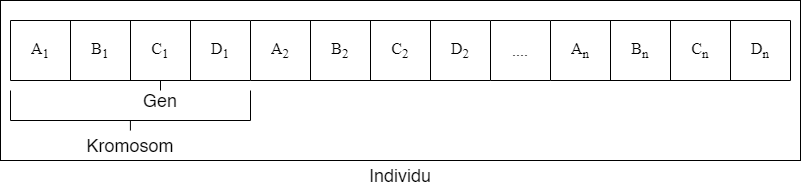
\includegraphics[scale=0.5]{gambar/kromosom.png}
    % Keterangan gambar yang diinputkan
    \caption{Desain Kromosom}
    % Label referensi dari gambar yang diinputkan
    \label{fig:kromosom}
\end{figure}\\
  Keterangan:\\
  A = Dosen\\
  B = Mata Kuliah\\
  C = Ruangan\\
  D = Waktu\\
  n = Kromosom ke-n

Sedangkan untuk proses pengkodean gen digunakan metode permutasi dengan \linebreak membangkitkan angka secara acak yang mewakili urutan masing-masing data yang \linebreak direpresentasikan oleh masing-masing gen.

\subsection{Inisialisasi Populasi}
Hal pertama yang dilakukan dalam program penjadwalan ini adalah pembangkitan \linebreak individu-individu induk sesuai dengan desain kromosom yang telah dibuat sebelumnya. Individu ini berbentuk \emph{nested list} yang berisi list gen didalam list kromosom dalam satu kesatuan individu.  
\begin{lstlisting}[
  language=Python,
  caption={Fungsi pembangkitan individu},
  label={lst:Populasi}
  ]
  def create_individu():
  individu = [[random.randint(1, len(Dosen.dosen)), 
              i+1,
               random.randint(1, len(Ruang.ruang)),
               random.randint(1, len(Waktu.waktu))
               ] 
              for i in range (len(Matkul.matkul))]
  return individu
\end{lstlisting}
Panjang kromosom untuk masing-masing individu sesuai dengan banyaknya mata kuliah yang akan dilaksanakan dalam satu semester perkuliahan.
\subsection{Evaluasi Fitness}
  
  Individu-individu yang ada dievaluasi dengan fungsi fitness untuk menentukan kecocokan dengan batasan yang telah ditentukan sebelumnya. 
  Fungsi fitness yang digunakan adalah sebagai berikut:
  
  \begin{equation}
    \label{eq:fitness2}
    \mathbf{Fitness} = \frac{1}{(1 + (F1 + F2 + \cdot \cdot \cdot +  Fn))}\; 
  \end{equation}\\
  Keterangan:\\
  Fn = Banyaknya Konflik\\
  n  = Batasan ke-n\\

  Fungsi \ref{eq:fitness2} akan menghitung banyaknya konflik yang ada pada satu individu. Konflik ini berupa pelanggaran pada batasan yang telah ditentukan sebelumnya.
  Batasan-batasan tersebut antara lain:
  \begin{enumerate}[nolistsep]
    \item Satu mata kuliah hanya bisa diselenggarakan satu kali dalam satu minggu
    \item Satu ruangan hanya bisa dipakai satu kali dalam satu waktu
    \item Satu dosen hanya bisa mengajar satu kali dalam satu waktu
    \item Jumlah peserta perkuliahan tidak boleh melebihi kapasitas ruangan
  \end{enumerate} 
 Pada proses penghitungan konflik, nilai 1 ditambahkan untuk menghindari hasil tak hingga ketika tidak ada pelanggaran sama sekali. 
 Semakin besar nilai fitness yang dihasilkan, maka semakin baik individu tersebut dan semakin cocok dengan hasil penjadwalan yang diharapkan. 
\subsection{Pemilihan Individu Induk}
  
  Individu-individu yang telah melalui proses evaluasi dipilih untuk dijadikan sebagai \linebreak induk untuk proses crossover.
  Metode yang digunakan dalam proses seleksi ini adalah metode \linebreak rangking, dimana individu dengan fitness terbaik digunakan sebagai individu induk untuk proses selanjutnya. 
  Proses pemilihan individu induk dilakukan dengan program dibawah ini:
  \begin{lstlisting}[
    language=Python,
    caption={Fungsi pemilihan individu induk},
    label={lst:selection}
    ]
    def selection(a,b,c,d,e,f):
      pop = [a,b,c,d,e,f]

      sorted_pop = sorted(pop, key=lambda x: fitness(x), reverse=True)
      
      x1 = sorted_pop[0]
      x2 = sorted_pop[1]
      fit = fitness(x1)

    return x1,x2,fitness(x1)
  \end{lstlisting}
  Fungsi ini akan mengembalikan 2 individu terbaik dari total 6 individu yang dimasukkan, sekaligus mengembalikan nilai fitness dari individu terbaik. 
  Individu yang dikembalikan ini digunakan untuk proses \emph{loop} berikutnya dan nilai fitness ini digunakan untuk kebutuhan penghentian proses penjadwalan otomatis ini.
\subsection{\emph{Crossover}}
  
Crossover atau pindah silang adalah salah satu komponen algoritma genetika yang \linebreak berfungsi untuk mendapatkan solusi dengan melakukan pindah silang kromosom-kromosom dari dua buah individu yang biasa disebut \emph{parent}. 
Proses ini akan menghasilkan 2 individu baru yang disebut dengan \emph{child}. Proses \emph{crossover} dilakukan dengan skema sesuai gambar dibawah ini:
% \begin{lstlisting}[
%   language=Python,
%   caption={Fungsi crossover},
%   label={lst:crossover},
%   ]
%   def crossover(a,b):
%     a = list(a)
%     b = list(b)
%     n = random.randint(1, (len(a)-1))
%     m = random.randint(n, (len(a)-1))

%     for i in range (n, m):
%       a[i],b[i] = b[i],a[i]

%   return a,b
% \end{lstlisting}
\begin{figure} [ht] \centering
  % Nama dari file gambar yang diinputkan
  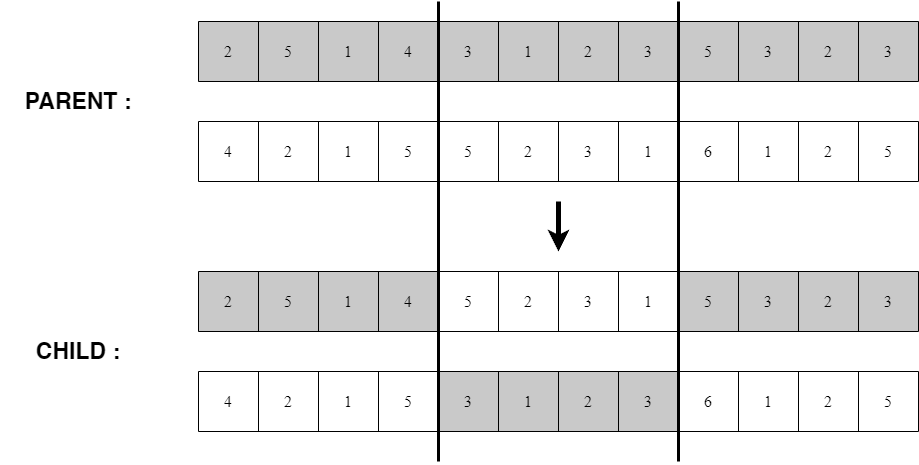
\includegraphics[scale=0.4]{gambar/cross.png}
  % Keterangan gambar yang diinputkan
  \caption{Two Points Crossover}
  % Label referensi dari gambar yang diinputkan
  \label{fig:cross}
\end{figure}

Pada proses crossover ini digunakan 2 titik crossover berupa angka yang dibangkitkan secara random.
Kromosom yang berada diantara 2 titik tersebut, dipindahkan antara satu induk dengan induk yang lain sehingga menghasilkan 2 individu baru.
\emph{Child} atau individu baru yang dihasilkan dari proses ini akan diteruskan ke proses mutasi.

\subsection{Mutasi}
  
  Mutasi merupakan proses dalam algoritma genetika yang bertujuan untuk mengubah \linebreak isi gen dalam sebuah kromosom secara acak. 
  Tidak semua individu baru hasil crossover \linebreak mengalami proses mutasi. 
  Individu-individu baru akan mengalami mutasi atau tidak, \linebreak ditentukan oleh probabilitas mutasi dari proses algoritma genetika yang telah ditentukan sebelumnya. 
  Proses mutasi dilakukan dengan program berikut ini:
  \begin{lstlisting}[
    language=Python,
    caption={Fungsi mutasi},
    label={lst:mutasi},
    ]
    def gA(a,b,rate):
      generation = 0
      score = 0.00
      while True:
        if generation == 200000 or score == 1.00:
          
          break
        else:
          print("Generation: ", generation)
          c,d = crossover(a,b)
          e,f = mutate(c,d,rate)
          a,b,fit = selection(a,b,c,d,e,f)
          
          print("Fitness a:", fitness(a))
          print("Fitness b:", fitness(b))
          print("\n")
          score = fit
          generation = generation+1

      return a    
  \end{lstlisting}
  Untuk menentukan proses mutasi berjalan atau tidak, dilakukan dengan cara membangkitkan angka secara acak antara 0 hingga 1. 
  Jika angka yang dibangkitkan memiliki nilai dibawah probabilitas mutasi, maka proses mutasi akan terjadi.
  \begin{figure} [ht] \centering
    % Nama dari file gambar yang diinputkan
    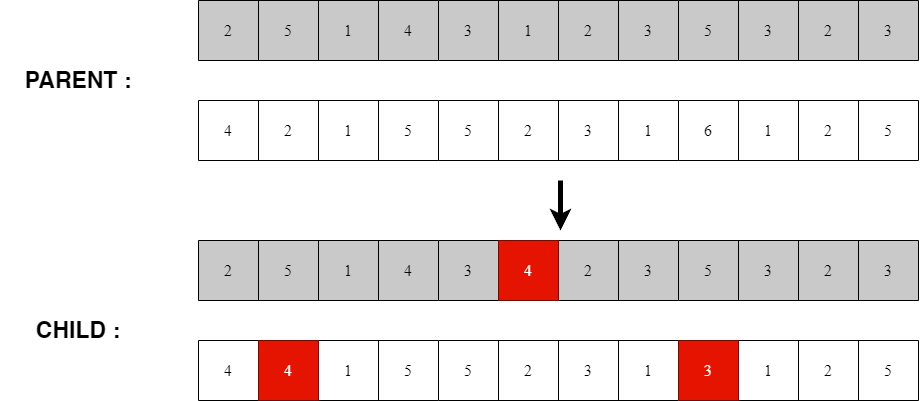
\includegraphics[scale=0.4]{gambar/mutation.png}
    % Keterangan gambar yang diinputkan
    \caption{Proses Mutasi}
    % Label referensi dari gambar yang diinputkan
    \label{fig:mutate}
  \end{figure}

  Proses mutasi akan membangkitkan ulang nilai gen-gen pada sebuah cromosom secara acak (Gambar \ref{fig:mutate}). Penentuan posisi kromosom yang dimutasi juga dilakukan secara acak dengan membangkitkan angka dalam jangkauan tertentu. 
  Proses mutasi ini menghasilkan 2 individu baru.
  \subsection{Kriteria Penghentian}
  
  Proses algoritma genetika hanya akan berhenti jika telah memenuhi kriteria penghentian yang telah ditentukan sebelumnya. 
  Kriteria penghentian ini dapat berupa nilai fitness tertentu, atau jumlah iterasi tertentu. 
  Jika nilai fitness telah terpenuhi atau jumlah iterasi telah terlewati, maka proses algoritma genetika akan berhenti.

\section{Bahan dan Peralatan yang Digunakan}
Dalam penelitian ini akan digunakan beberapa perangkat yang dibutuhkan untuk menunjang berjalannya penelitian dengan baik.
Berikut merupakan hardware dan software yang digunakan dalam melakukan proses pembuatan program sekaligus pengujian program yang digunakan pada penelitian ini.
\subsection{\emph{Hardware}}
Perangkat komputer yang digunakan untuk pengerjaan tugas akhir ini antara lain \emph{Asus TUF FX 505 DT} dengan spesifikasi \emph{AMD Ryzen 5 R5-3550H Processor, GeForce GTX 1650 Graphics, 16GB DDR4, 1TB HDD, 512GB SSD,} dan \emph{Windows 11 64-bit}.
\subsection{\emph{Software}}
\emph{Software} yang digunakan dalam penelitian ini adalah \emph{Jupyter Notebook} dan \emph{Google Colab}.

% \section{Urutan Pelaksanaan Penelitian}
% % Ubah tabel berikut sesuai dengan isi dari rencana kerja
% \newcommand{\w}{}
% \newcommand{\G}{\cellcolor{gray}}
% \begin{table}[h!]
%   \caption{Tabel timeline}
%   \label{tb:timeline}
%   \begin{tabular}{|p{3.5cm}|c|c|c|c|c|c|c|c|c|c|c|c|c|c|c|c|}

%     \hline
%     \multirow{2}{*}{Kegiatan} & \multicolumn{16}{|c|}{Minggu} \\
%     \cline{2-17} &
%     1 & 2 & 3 & 4 & 5 & 6 & 7 & 8 & 9 & 10 & 11 & 12 & 13 & 14 & 15 & 16 \\
%     \hline

%     % Gunakan \G untuk mengisi sel dan \w untuk mengosongkan sel
%     Studi Literatur &
%     \G & \G & \w & \w & \w & \w & \w & \w & \w & \w & \w & \w & \w & \w & \w & \w \\
%     \hline

%     Pengumpulan Data &
%     \w & \G & \G & \w & \w & \w & \w & \w & \w & \w & \w & \w & \w & \w & \w & \w \\
%     \hline

%     Preprocessing Data &
%     \w & \w & \G & \G & \G & \w & \w & \w & \w & \w & \w & \w & \w & \w & \w & \w \\
%     \hline

%     Pembuatan Program &
%     \w & \w & \w & \w & \G & \G & \G & \G & \G & \G & \G & \G & \w & \w & \w & \w \\
%     \hline

%     Pengujian Program &
%     \w & \w & \w & \w & \w & \w & \w & \w & \w & \w & \w & \G & \G & \G & \w & \w \\
%     \hline

%     Penyusunan \linebreak Laporan &
%     \G & \G & \G & \G & \G & \G & \G & \G & \G & \G & \G & \G & \G & \G & \G & \G \\
%     \hline

%   \end{tabular}
% \end{table}
% \section{Bahan dan Alat yang Digunakan}
%   \label{sec:bahan dan alat}

% Alat diimplementasikan dengan \lipsum[1]

% Contoh pembuatan potongan kode
% \begin{lstlisting}[
%   language=C++,
%   caption={Program halo dunia.},
%   label={lst:halodunia}
% ]
% #include <iostream>

% int main() {
%     std::cout << "Halo Dunia!";
%     return 0;
% }
% \end{lstlisting}

% \lipsum[2-3]

% % Contoh input potongan kode dari file
% \lstinputlisting[
%   language=Python,
%   caption={Program perhitungan bilangan prima.},
%   label={lst:bilanganprima}
% ]{program/bilangan-prima.py}

% \lipsum[4]
